%% ==========================================================================
%% Appendix: Supplementary Tables and Figures
%% Project 907 — "The Economics of Extended Play"
%% ==========================================================================

\appendix
\section*{Online Appendix A: Supplementary Tables and Figures}
\addcontentsline{toc}{section}{Online Appendix A: Supplementary Tables and Figures}

\setcounter{table}{0}
\renewcommand{\thetable}{A\arabic{table}}
\setcounter{figure}{0}
\renewcommand{\thefigure}{A\arabic{figure}}

%% --------------------------------------------------------------------------
%% Table A1: Full Event Study Coefficients
%% --------------------------------------------------------------------------

\begin{table}[htbp]
\centering
\begin{threeparttable}
\caption{Event Study Coefficients: Full Results}
\label{tab:event_study_full}
\begin{tabular}{lccccc}
\toprule
Season & $\hat{\beta}$ & SE & $t$ & $p$ & 95\% CI \\
\midrule
2017--18 & $-0.388^{***}$ & (0.082) & $-4.72$ & 0.000 & [$-0.549$, $-0.227$] \\
2018--19 & $-0.144$ & (0.085) & $-1.69$ & 0.091 & [$-0.310$, $+0.023$] \\
2019--20 & $-0.415^{***}$ & (0.088) & $-4.72$ & 0.000 & [$-0.587$, $-0.243$] \\
2020--21 & $-0.512^{***}$ & (0.083) & $-6.17$ & 0.000 & [$-0.675$, $-0.349$] \\
2021--22 & $-0.206^{**}$ & (0.090) & $-2.30$ & 0.022 & [$-0.381$, $-0.030$] \\
\addlinespace
2022--23 & \multicolumn{5}{c}{\textit{--- Reference period ---}} \\
\addlinespace
2023--24 & $+0.522^{***}$ & (0.099) & $+5.29$ & 0.000 & [$+0.329$, $+0.716$] \\
2024--25 & $+0.374^{***}$ & (0.097) & $+3.84$ & 0.000 & [$+0.183$, $+0.565$] \\
2025--26 & $+0.464^{***}$ & (0.127) & $+3.65$ & 0.000 & [$+0.215$, $+0.713$] \\
\bottomrule
\end{tabular}
\begin{tablenotes}[flushleft]
\footnotesize
\item \textit{Notes:} Event study estimates from a TWFE regression of second-half
stoppage time on season indicators interacted with the treated-league dummy, with
league and season fixed effects. The reference period is 2022--23 (the last
pre-treatment season). Robust standard errors (HC1) in parentheses.
$^{*}p<0.10$, $^{**}p<0.05$, $^{***}p<0.01$.
\end{tablenotes}
\end{threeparttable}
\end{table}

%% --------------------------------------------------------------------------
%% Table A2: Specification Curve Full Results
%% --------------------------------------------------------------------------

\begin{table}[htbp]
\centering
\begin{threeparttable}
\caption{Specification Curve: Full Results (36 Specifications)}
\label{tab:spec_curve_full}
\small
\begin{tabular}{clllllrrrr}
\toprule
Spec & DV & FE & Sample & Cluster & $\hat{\beta}$ & SE & $p$ & $N$ & Sig. \\
\midrule
\addlinespace
\multicolumn{10}{l}{\textit{Panel A: 2H stoppage time}} \\
\addlinespace[3pt]
1 & 2H & League & Full & HC1 & 1.564 & 0.037 & 0.000 & 36,663 & $\checkmark$ \\
2 & 2H & League & Full & Cluster & 1.564 & 0.233 & 0.000 & 36,663 & $\checkmark$ \\
3 & 2H & League & No COVID & HC1 & 1.522 & 0.039 & 0.000 & 28,644 & $\checkmark$ \\
4 & 2H & League & No COVID & Cluster & 1.522 & 0.244 & 0.000 & 28,644 & $\checkmark$ \\
5 & 2H & League & Post-2017 & HC1 & 1.564 & 0.037 & 0.000 & 33,452 & $\checkmark$ \\
6 & 2H & League & Post-2017 & Cluster & 1.564 & 0.233 & 0.000 & 33,452 & $\checkmark$ \\
7 & 2H & Season & Full & HC1 & 0.867 & 0.049 & 0.000 & 36,663 & $\checkmark$ \\
8 & 2H & Season & Full & Cluster & 0.867 & 0.522 & 0.097 & 36,663 & \\
9 & 2H & Season & No COVID & HC1 & 0.867 & 0.049 & 0.000 & 28,644 & $\checkmark$ \\
10 & 2H & Season & No COVID & Cluster & 0.867 & 0.522 & 0.097 & 28,644 & \\
11 & 2H & Season & Post-2017 & HC1 & 0.867 & 0.049 & 0.000 & 33,452 & $\checkmark$ \\
12 & 2H & Season & Post-2017 & Cluster & 0.867 & 0.522 & 0.097 & 33,452 & \\
13 & 2H & Lg$\times$Sn & Full & HC1 & 0.734 & 0.053 & 0.000 & 36,663 & $\checkmark$ \\
14 & 2H & Lg$\times$Sn & Full & Cluster & 0.734 & 0.278 & 0.008 & 36,663 & $\checkmark$ \\
15 & 2H & Lg$\times$Sn & No COVID & HC1 & 0.648 & 0.056 & 0.000 & 28,644 & $\checkmark$ \\
16 & 2H & Lg$\times$Sn & No COVID & Cluster & 0.648 & 0.261 & 0.013 & 28,644 & $\checkmark$ \\
17 & 2H & Lg$\times$Sn & Post-2017 & HC1 & 0.727 & 0.053 & 0.000 & 33,452 & $\checkmark$ \\
18 & 2H & Lg$\times$Sn & Post-2017 & Cluster & 0.727 & 0.278 & 0.009 & 33,452 & $\checkmark$ \\
\addlinespace
\multicolumn{10}{l}{\textit{Panel B: Total stoppage time}} \\
\addlinespace[3pt]
19 & Total & League & Full & HC1 & 2.666 & 0.053 & 0.000 & 27,975 & $\checkmark$ \\
20 & Total & League & Full & Cluster & 2.666 & 0.381 & 0.000 & 27,975 & $\checkmark$ \\
21 & Total & League & No COVID & HC1 & 2.630 & 0.055 & 0.000 & 21,253 & $\checkmark$ \\
22 & Total & League & No COVID & Cluster & 2.630 & 0.384 & 0.000 & 21,253 & $\checkmark$ \\
23 & Total & League & Post-2017 & HC1 & 2.666 & 0.053 & 0.000 & 27,381 & $\checkmark$ \\
24 & Total & League & Post-2017 & Cluster & 2.666 & 0.381 & 0.000 & 27,381 & $\checkmark$ \\
25 & Total & Season & Full & HC1 & 0.663 & 0.072 & 0.000 & 27,975 & $\checkmark$ \\
26 & Total & Season & Full & Cluster & 0.663 & 0.640 & 0.301 & 27,975 & \\
27 & Total & Season & No COVID & HC1 & 0.663 & 0.072 & 0.000 & 21,253 & $\checkmark$ \\
28 & Total & Season & No COVID & Cluster & 0.663 & 0.640 & 0.301 & 21,253 & \\
29 & Total & Season & Post-2017 & HC1 & 0.663 & 0.072 & 0.000 & 27,381 & $\checkmark$ \\
30 & Total & Season & Post-2017 & Cluster & 0.663 & 0.640 & 0.301 & 27,381 & \\
31 & Total & Lg$\times$Sn & Full & HC1 & 1.200 & 0.080 & 0.000 & 27,975 & $\checkmark$ \\
32 & Total & Lg$\times$Sn & Full & Cluster & 1.200 & 0.409 & 0.003 & 27,975 & $\checkmark$ \\
33 & Total & Lg$\times$Sn & No COVID & HC1 & 1.196 & 0.084 & 0.000 & 21,253 & $\checkmark$ \\
34 & Total & Lg$\times$Sn & No COVID & Cluster & 1.196 & 0.412 & 0.004 & 21,253 & $\checkmark$ \\
35 & Total & Lg$\times$Sn & Post-2017 & HC1 & 1.190 & 0.080 & 0.000 & 27,381 & $\checkmark$ \\
36 & Total & Lg$\times$Sn & Post-2017 & Cluster & 1.190 & 0.409 & 0.004 & 27,381 & $\checkmark$ \\
\bottomrule
\end{tabular}
\begin{tablenotes}[flushleft]
\footnotesize
\item \textit{Notes:} Full specification curve results. Each row is one OLS specification
with the indicated dependent variable, fixed effects, sample restriction, and standard
error type. ``Lg$\times$Sn'' denotes league-season interacted fixed effects.
``Cluster'' denotes standard errors clustered at the league level (15 clusters).
``HC1'' denotes heteroskedasticity-robust standard errors. ``No COVID'' drops the
2019--20 and 2020--21 seasons. ``Post-2017'' drops pre-2017--18 seasons.
$\checkmark$ denotes $p<0.05$. Median coefficient across all 36 specifications:
$+1.028$; 83\% significant at $p<0.05$; 100\% positive.
\end{tablenotes}
\end{threeparttable}
\end{table}

%% --------------------------------------------------------------------------
%% Table A3: League-by-League DiD Estimates
%% --------------------------------------------------------------------------

\begin{table}[htbp]
\centering
\begin{threeparttable}
\caption{Heterogeneous Treatment Effects by League}
\label{tab:league_did}
\begin{tabular}{lcccccc}
\toprule
League & $\hat{\beta}_{\text{DiD}}$ & SE & $p$ & 95\% CI & $N$ \\
\midrule
Premier League & $+1.310^{***}$ & (0.089) & 0.000 & [$+1.135$, $+1.484$] & 24,596 \\
Bundesliga & $+0.934^{***}$ & (0.095) & 0.000 & [$+0.748$, $+1.121$] & 23,888 \\
Ligue~1 & $+0.958^{***}$ & (0.087) & 0.000 & [$+0.787$, $+1.129$] & 24,269 \\
Serie~A & $-0.094$ & (0.080) & 0.239 & [$-0.251$, $+0.063$] & 24,559 \\
La Liga & $+0.635^{***}$ & (0.094) & 0.000 & [$+0.452$, $+0.818$] & 24,559 \\
\midrule
Pooled (all Big~5) & $+0.734^{***}$ & (0.053) & 0.000 & [$+0.631$, $+0.838$] & 36,663 \\
\bottomrule
\end{tabular}
\begin{tablenotes}[flushleft]
\footnotesize
\item \textit{Notes:} League-specific DiD estimates. Each row reports the coefficient
on Post~$\times$~Treated from a separate regression including only the specified
treated league and all control leagues, with league and season fixed effects.
The pooled estimate includes all five treated leagues. Robust standard errors
(HC1) in parentheses. Joint test for heterogeneity across leagues:
$F(4, 15344) = 51.12$, $p = 0.000$. The Serie~A null result is consistent with
Italian football's pre-existing tradition of generous stoppage time (pre-treatment
mean $\approx 5.2$ min vs.\ Big~5 average of $5.0$ min), leaving less room for
upward adjustment. $^{*}p<0.10$, $^{**}p<0.05$, $^{***}p<0.01$.
\end{tablenotes}
\end{threeparttable}
\end{table}

%% --------------------------------------------------------------------------
%% Table A4: Referee Compliance (Within-Referee Fixed Effects)
%% --------------------------------------------------------------------------

\begin{table}[htbp]
\centering
\begin{threeparttable}
\caption{Referee Compliance with the FIFA Directive}
\label{tab:referee_compliance}
\begin{tabular}{lcc}
\toprule
& \multicolumn{2}{c}{Dep.\ var.: 2H Stoppage (min)} \\
\cmidrule(lr){2-3}
& (1) Pooled DiD & (2) Within-Referee FE \\
\midrule
Post $\times$ Treated & $+0.602^{***}$ & $+1.484^{***}$ \\
& (0.061) & (0.040) \\
\addlinespace
League FE & \checkmark & \\
Season FE & \checkmark & \checkmark \\
Referee FE & & \checkmark \\
\midrule
Observations & 24,470 & 19,258 \\
$R^2$ & 0.156 & 0.071 \\
Referees & 485 & 485 \\
\bottomrule
\end{tabular}
\begin{tablenotes}[flushleft]
\footnotesize
\item \textit{Notes:} Column~(1) reports the pooled DiD specification with league
and season fixed effects on referee-match observations. Column~(2) adds
within-referee fixed effects, absorbing time-invariant referee heterogeneity
(e.g., leniency). The sample covers 485 referees across 10 leagues. The
within-referee estimate exceeds the pooled estimate, suggesting that between-referee
compositional changes attenuate the pooled effect. Robust standard errors
(HC1) in parentheses. $^{*}p<0.10$, $^{**}p<0.05$, $^{***}p<0.01$.
\end{tablenotes}
\end{threeparttable}
\end{table}

%% --------------------------------------------------------------------------
%% Table A5: Mechanism Decomposition (Gelbach 2016)
%% --------------------------------------------------------------------------

\begin{table}[htbp]
\centering
\begin{threeparttable}
\caption{Mechanism Decomposition: Gelbach (2016) Analysis}
\label{tab:mechanism_gelbach}
\begin{tabular}{lrrrr}
\toprule
Channel & $\hat{\pi}$ (DiD$\to$Channel) & $\hat{\gamma}$ (Channel coef.) & $\hat{\delta} = \hat{\gamma} \times \hat{\pi}$ & \% of base \\
\midrule
\addlinespace
\multicolumn{5}{l}{\textit{Panel A: Full DiD with control leagues ($N = 24{,}469$)}} \\
\addlinespace[3pt]
\quad Fouls & $+0.803^{***}$ & $+0.013^{***}$ & $+0.011$ & 1.8\% \\
\quad Cards & $-0.192^{***}$ & $+0.189^{***}$ & $-0.036$ & $-6.0$\% \\
\quad Shots & $+0.304^{*}$ & $+0.020^{***}$ & $+0.006$ & 1.0\% \\
\quad Corners & $-0.180$ & $+0.016^{***}$ & $-0.002$ & $-0.4$\% \\
\quad Close match & $+0.002$ & $+1.075^{***}$ & $+0.002$ & 0.4\% \\
\midrule
Observable channels (total) & & & $-0.020$ & $-3.2$\% \\
Referee discretion (residual) & & & $+0.622$ & 103.2\% \\
\midrule
Base DiD effect & & & $+0.602$ & 100.0\% \\
\addlinespace[6pt]
\multicolumn{5}{l}{\textit{Panel B: Big~5 only with late goals ($N = 15{,}337$)}} \\
\addlinespace[3pt]
\quad Fouls & & & $-0.022$ & $-1.4$\% \\
\quad Cards & & & $+0.022$ & 1.3\% \\
\quad Shots & & & $+0.003$ & 0.2\% \\
\quad Corners & & & $-0.007$ & $-0.4$\% \\
\quad Close match & & & $-0.003$ & $-0.2$\% \\
\quad Late goals (90$+$) & $+0.056^{***}$ & $+1.184^{***}$ & $+0.066$ & 4.1\% \\
\midrule
Observable channels (total) & & & $+0.058$ & 3.6\% \\
Referee discretion (residual) & & & $+1.562$ & 96.4\% \\
\midrule
Base pre/post effect & & & $+1.620$ & 100.0\% \\
\bottomrule
\end{tabular}
\begin{tablenotes}[flushleft]
\footnotesize
\item \textit{Notes:} Gelbach (2016) decomposition of the treatment effect into
observable match-event channels and a residual (referee discretion). $\hat{\pi}$
is the DiD effect of treatment on the channel variable. $\hat{\gamma}$ is the
channel's coefficient in the full model. $\hat{\delta} = \hat{\gamma} \times
\hat{\pi}$ is each channel's contribution to the base effect. Panel~A uses
the full DiD sample (treated + control leagues). Panel~B restricts to Big~5
leagues (pre/post design) and adds late goals ($>$90~min) as a channel,
unavailable for control leagues. The residual captures referee discretion ---
the portion of extra stoppage time not mechanically explained by observable
match events. $^{*}p<0.10$, $^{**}p<0.05$, $^{***}p<0.01$.
\end{tablenotes}
\end{threeparttable}
\end{table}

%% --------------------------------------------------------------------------
%% Table A6: Data Coverage Matrix
%% --------------------------------------------------------------------------

\begin{table}[htbp]
\centering
\begin{threeparttable}
\caption{Data Coverage: Leagues $\times$ Seasons (2H Stoppage Time)}
\label{tab:coverage_matrix}
\small
\begin{tabular}{lrrrl}
\toprule
League & Pre & Post & Total & Treatment \\
\midrule
\addlinespace
\multicolumn{5}{l}{\textit{Treated (Big~5)}} \\
\addlinespace[3pt]
\quad Bundesliga (D1) & 1,787 & 799 & 2,586 & Treated \\
\quad Premier League (E0) & 2,276 & 1,018 & 3,294 & Treated \\
\quad Ligue~1 (F1) & 2,168 & 799 & 2,967 & Treated \\
\quad Serie~A (I1) & 2,262 & 995 & 3,257 & Treated \\
\quad La Liga (SP1) & 2,271 & 986 & 3,257 & Treated \\
\addlinespace
\multicolumn{5}{l}{\textit{Control}} \\
\addlinespace[3pt]
\quad Belgian Pro League (B1) & 1,179 & 393 & 1,572 & Control \\
\quad 2.\ Bundesliga (D2) & 2,354 & 302 & 2,656 & Control \\
\quad Championship (E1) & 3,287 & 1,466 & 4,753 & Control \\
\quad Ligue~2 (F2) & 1,457 & 380 & 1,837 & Control \\
\quad Greek Super League (G1) & 1,103 & 303 & 1,406 & Control \\
\quad Serie~B (I2) & 2,268 & 448 & 2,716 & Control \\
\quad Eredivisie (N1) & 920 & 810 & 1,730 & Control \\
\quad Primeira Liga (P1) & 1,827 & 801 & 2,628 & Control \\
\quad Scottish Premiership (SC0) & 836 & 171 & 1,007 & Control \\
\quad Segunda Divisi\'{o}n (SP2) & 997 & 0 & 997 & Control \\
\midrule
\textit{Total} & 26,992 & 9,671 & 36,663 & \\
\bottomrule
\end{tabular}
\begin{tablenotes}[flushleft]
\footnotesize
\item \textit{Notes:} Match counts by league for the second-half stoppage time
analysis sample. ``Pre'' denotes seasons before 2023--24; ``Post'' denotes
2023--24 onward (post-FIFA directive). Treated leagues are the Big~5 European
leagues subject to the PGMOL unified stoppage-time directive. Control leagues
are second-division or smaller top-flight leagues not directly targeted by the
directive. The Super Lig (T1) is excluded from match-level regressions due to
near-zero stoppage-time coverage; it enters as a never-treated control in
player-level analyses. The Segunda Divisi\'{o}n (SP2) has zero post-period
observations due to data availability.
\end{tablenotes}
\end{threeparttable}
\end{table}

%% --------------------------------------------------------------------------
%% Figure A1: Placebo Null Distribution
%% --------------------------------------------------------------------------

\begin{figure}[htbp]
\centering

\includegraphics[width=0.85\textwidth]{../output/a07_placebo_null_dist.png}
\caption{Permutation Inference: Null Distribution of Placebo DiD Estimates}
\label{fig:placebo_null}
\begin{minipage}{0.85\textwidth}
\footnotesize
\textit{Notes:} Histogram of 1,000 placebo DiD estimates obtained by randomly
reassigning treatment status across leagues. The vertical dashed line marks
the observed DiD estimate ($\hat{\beta} = +0.734$). Permutation $p$-value
(two-sided): $0.043$. The observed effect lies in the extreme right tail of
the null distribution (null mean $= -0.037$, null SD $= 0.368$), confirming
that the treatment effect is unlikely to arise from chance.
\end{minipage}
\end{figure}

%% --------------------------------------------------------------------------
%% Figure A2: League-Level Event Studies
%% --------------------------------------------------------------------------

\begin{figure}[htbp]
\centering
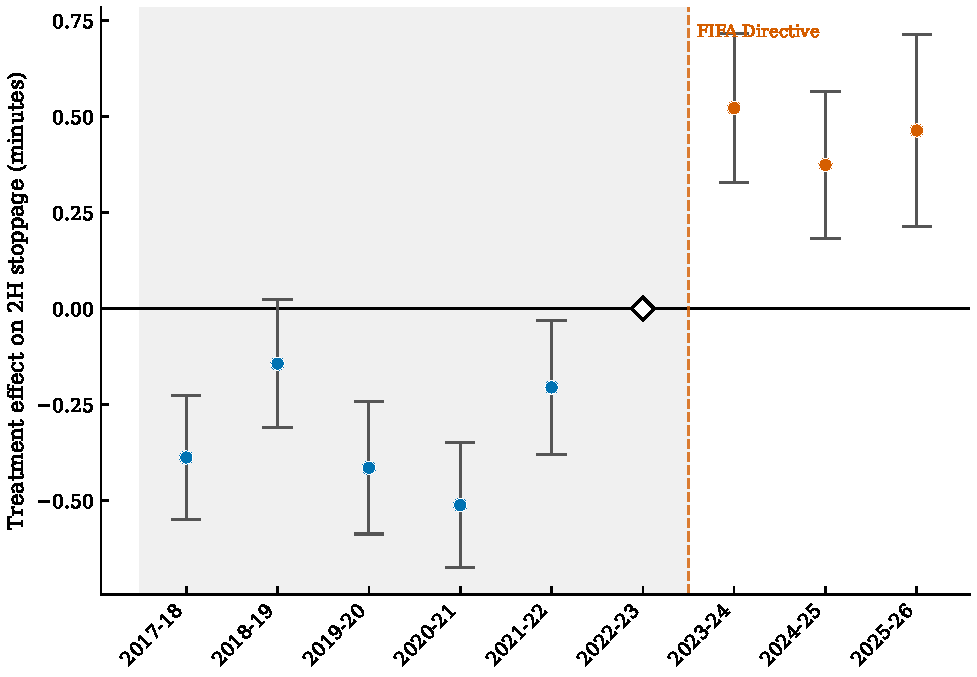
\includegraphics[width=0.85\textwidth]{../output/figures/fig1_event_study.pdf}
\caption{Event Study: Dynamic Treatment Effects by Season}
\label{fig:event_study_appendix}
\begin{minipage}{0.85\textwidth}
\footnotesize
\textit{Notes:} Event study coefficients and 95\% confidence intervals from
a TWFE regression of second-half stoppage time on season-by-treatment indicators.
The reference period is 2022--23. Pre-treatment coefficients test for parallel
trends; post-treatment coefficients capture the dynamic treatment effect. The
positive and stable post-treatment coefficients ($+0.37$ to $+0.52$) indicate
a persistent effect of the FIFA directive with no evidence of attenuation.
Robust standard errors (HC1).
\end{minipage}
\end{figure}
